\documentclass[a4paper,12pt]{article}
\usepackage[utf8]{inputenc}
\usepackage[a4paper, margin=1in]{geometry}
\usepackage{graphicx}
\usepackage{caption}
\usepackage{amsmath}
\usepackage{amssymb}
\usepackage{float}
\usepackage{mathabx}
\usepackage{stackengine}
\usepackage{ragged2e}    % Para control de justificación
\justifying

\setlength{\parindent}{0pt}
\setlength{\parskip}{1em}
\linespread{1.2}

\newcommand{\Vbar}{\stackon[-1ex]{V}{\rule{1.5ex}{0.3pt}}}


\title{Lecture 4: Blood Flow in Arteries}
\author{}
\date{}

\begin{document}

\maketitle

\section*{Introduction}

The cardiovascular system is a complex network responsible for the transport of blood throughout the body, governed by dynamic interactions between flow, pressure, and vessel elasticity. To better understand and approximate the behavior of blood flow in this system, we develop a mathematical model by progressively linking three increasingly sophisticated fluid dynamics models.

We begin with the classical \textbf{Hagen--Poiseuille flow}, which describes steady, laminar flow through a rigid, cylindrical pipe. Although simplistic, this model serves as a foundational reference for understanding viscous flow behavior under constant pressure gradients.

Next, we introduce \textbf{time-dependent flow}, incorporating a harmonic oscillation in the pressure gradient. This allows us to account for the pulsatile nature of blood flow driven by the rhythmic contractions of the heart, although it still assumes rigid vessel walls.

Finally, we extend the model to consider \textbf{flexible-walled tubes} subjected to oscillatory pressure fields. This last approach offers the most realistic approximation of actual physiological conditions in the cardiovascular system, where vessel compliance and wave propagation play a crucial role in shaping blood flow dynamics.

Throughout, we maintain assumptions relevant to large vessels such as the aorta, including laminar flow and axisymmetry. Our ultimate goal is to construct a model that not only captures the essential physics but also aligns with physiological observations.

\section{Fixed Pipe Flow}

\begin{figure}[H]
\centering
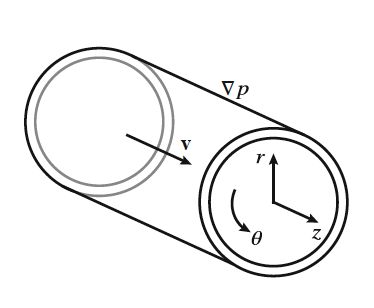
\includegraphics[width=0.35\textwidth]{hagen-poiseuille.png}
\caption{Scheme of the flow through a fixed wall pipe}
\end{figure}

From this point on, we adopt the following assumptions:

\begin{itemize}
    \item Newtonian flow $\left(\tau \propto \frac{\partial \vec{v}}{\partial \vec{r}}\right)$
    \item No-slip condition $\left(\vec{v}|_{\text{walls}}=0\right)$
    \item Laminar flow $(Re \ll 1)$
    \item Fully developed (steady solution)
    \item Circular cross-section
\end{itemize}

\textit{Physiological context:} This model represents flow in large arteries under simplified conditions. While real arteries are pulsatile and elastic, this steady model allows us to understand the fundamental role of viscosity and velocity profile development.


The equations for the system are (in cylindrical coordinates):

\subsection*{Continuity Equation}


\textbf{1) Continuity (incompressibility):}

In cylindrical coordinates, the incompressibility condition is given by:

\[
\frac{1}{r} \frac{d}{dr}(r v_r) + \frac{1}{r} \frac{\partial v_\theta}{\partial \theta} + \frac{\partial v_z}{\partial z} = 0
\]

\medskip

Assuming axial flow only:
\[
\vec{v} = v_z \, \vec{e}_z \quad \Rightarrow \quad \frac{\partial v_z}{\partial z} = 0
\]

\[
\Rightarrow \quad v_r = v_\theta = 0 \quad \text{and} \quad \frac{\partial v_z}{\partial z} = 0
\]



\textbf{2) Navier--Stokes:}

\textbf{Radial component $(r)$:}

\[
\rho \left( \frac{\partial v_r}{\partial t} + v_r \frac{\partial v_r}{\partial r} + \frac{v_\theta}{r} \frac{\partial v_r}{\partial \theta} + v_z \frac{\partial v_r}{\partial z} - \frac{v_\theta^2}{r} \right)
= -\frac{\partial p}{\partial r} + \mu \left( \nabla^2 v_r - \frac{v_r}{r^2} - \frac{2}{r^2} \frac{\partial v_\theta}{\partial \theta} \right)
\]

\medskip

Assuming a purely axial flow:
\[
\vec{v} = (0, 0, v_z) \quad \Rightarrow \quad \frac{\partial p}{\partial r} = 0
\]

\bigskip

\textbf{Azimuthal component $(\theta)$:}

\[
\rho \left( \frac{\partial v_\theta}{\partial t} + v_r \frac{\partial v_\theta}{\partial r} + \frac{v_\theta}{r} \frac{\partial v_\theta}{\partial \theta} + v_z \frac{\partial v_\theta}{\partial z} + \frac{v_r v_\theta}{r} \right)
= -\frac{1}{r} \frac{\partial p}{\partial \theta}
+ \mu \left( \nabla^2 v_\theta - \frac{v_\theta}{r^2} + \frac{2}{r^2} \frac{\partial v_r}{\partial \theta} \right)
\]

\[
\Rightarrow \quad \frac{\partial p}{\partial \theta} = 0
\]

\bigskip

\textbf{Axial component $(z)$:}

\[
\rho \left( \frac{\partial v_z}{\partial t} + v_r \frac{\partial v_z}{\partial r} + \frac{v_\theta}{r} \frac{\partial v_z}{\partial \theta} + v_z \frac{\partial v_z}{\partial z} \right)
= -\frac{\partial p}{\partial z} + \mu \nabla^2 v_z
\]

Assuming:
\begin{itemize}
  \item Stationary flow: \( \frac{\partial v_z}{\partial t} = 0 \)
  \item Continuity: \( \frac{\partial v_z}{\partial z} = 0 \)
\end{itemize}

Then:

\[
0 = -\frac{\partial p}{\partial z} + \mu \left\{ \frac{1}{r} \frac{d}{dr} \left( r \frac{d v_z}{dr} \right) \right\}
\quad \Rightarrow \quad \frac{\partial p}{\partial z} = \mu \left( \frac{1}{r} \frac{d}{dr} \left( r \frac{d v_z}{dr} \right) \right)
\]

\textbf{Solving the differential equation:}

Integrating with respect to \( r \):

\[
\frac{1}{\mu} \frac{dp}{dz} = \frac{1}{r} \frac{d}{dr} \left( r \frac{d v_z}{dr} \right)
\]

\[
\int_0^r \left( \frac{1}{\mu} \frac{dp}{dz} \right) dr = r \frac{dv_z}{dr} \Rightarrow \frac{dv_z}{dr} = \frac{1}{\mu} \left( \frac{dp}{dz} \right) \frac{r}{2} + C_1
\]

\[
v_z(r) = \int \left( \frac{dp}{dz} \cdot \frac{r}{2\mu} + C_1 \right) dr
= \frac{1}{4\mu} \left( \frac{dp}{dz} \right) r^2 + C_1 \ln r + C_2
\]

\[
\boxed{
v_z(r) = \frac{1}{4\mu} \left( \frac{dp}{dz} \right) r^2 + C_1 \ln r + C_2
}
\]


\subsection*{Boundary Conditions and Hagen--Poiseuille Solution}

\textbf{Boundary conditions:}

At the center of the pipe ($r = 0$), we require the velocity to be finite. However:

\[
\ln(0) \rightarrow \infty \Rightarrow C_1 = 0 \text{ (must be null)}
\]

At the wall ($r = R$), we apply the no-slip condition:

\[
v_z|_{r=R} = 0 \Rightarrow \frac{1}{4\mu} \left( \frac{dp}{dz} \right) R^2 + C_2 = 0
\]

\[
\Rightarrow C_2 = -\frac{1}{4\mu} \left( \frac{dp}{dz} \right) R^2
\]

\bigskip

\textbf{Final expression for Hagen--Poiseuille flow:}

\[
\boxed{
v_z(r) = \frac{1}{4\mu} \left( \frac{dp}{dz} \right) \left( r^2 - R^2 \right)
}
\]

This represents a \textit{fully developed, laminar pipe flow}, characterized by a parabolic velocity profile.

\begin{figure}[H]
\centering
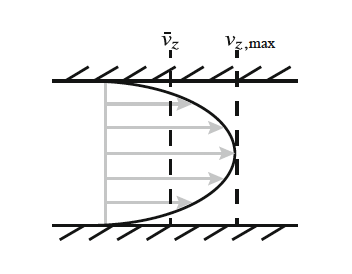
\includegraphics[width=0.35\textwidth]{velocity-hagen-poiseuille.png}
\caption{Velocity profile for Hagen-Poiseuille solution}
\end{figure}


\section{Pipe flow with oscillating pressure gradient}

Introducing a time dependence in the velocity profile. In this case through an oscillating pressure gradient $(\nabla p = f(t))$:

\subsection*{Axial component with oscillating pressure gradient}

From the Navier--Stokes equation (z-component):

\[
\rho \left( \frac{\partial v_z}{\partial t} + v_r \frac{\partial v_z}{\partial r} + \frac{v_\theta}{r} \frac{\partial v_z}{\partial \theta} + v_z \frac{\partial v_z}{\partial z} \right)
= -\frac{\partial p}{\partial z} + \mu \nabla^2 v_z
\]

\medskip

Assuming:
\begin{itemize}
    \item Axisymmetry: \( \frac{\partial}{\partial \theta} = 0 \)
    \item Fully developed: \( \frac{\partial v_z}{\partial z} = 0 \)
    \item Negligible radial/azimuthal velocity components: \( v_r = v_\theta = 0 \)
\end{itemize}

Then:

\[
\rho \frac{\partial v_z}{\partial t} = -\frac{\partial p}{\partial z} + \mu \frac{1}{r} \frac{\partial}{\partial r} \left( r \frac{\partial v_z}{\partial r} \right)
\]

Dividing by \( \rho \) and introducing kinematic viscosity \( \nu = \frac{\mu}{\rho} \):

\[
\frac{\partial v_z}{\partial t} = -\frac{1}{\rho} \frac{\partial p}{\partial z} + \nu \frac{1}{r} \frac{\partial}{\partial r} \left( r \frac{\partial v_z}{\partial r} \right)
\]

\medskip

Assume a harmonic variation in pressure:

\[
\frac{\partial p}{\partial z} = -\rho k e^{i \omega t} \qquad \text{with } \omega = 2\pi f
\]

\[
\Rightarrow \frac{\partial v_z}{\partial t} = k e^{i \omega t} + \nu \frac{1}{r} \frac{\partial}{\partial r} \left( r \frac{\partial v_z}{\partial r} \right)
\]

Or, expressed more explicitly:

\[
\frac{\partial v_z}{\partial t} = k e^{i \omega t} + \nu \left( \frac{\partial^2 v_z}{\partial r^2} + \frac{1}{r} \frac{\partial v_z}{\partial r} \right)
\]

\[
\boxed{
\frac{\partial v_z}{\partial t} = k e^{i \omega t} + \nu \left( \frac{\partial^2 v_z}{\partial r^2} + \frac{1}{r} \frac{\partial v_z}{\partial r} \right)
}
\]


\subsection*{Oscillatory Solution and Womersley Number}

For that equation, the full mathematical process is long and not the main focus here. So we directly present a solution that satisfies the differential equation:

\[
v_z(r,t) = \frac{k}{i\omega} e^{i\omega t} \left\{ 1 - \frac{J_0 \left( r \sqrt{-i \omega / \nu} \right)}{J_0 \left( R \sqrt{-i \omega / \nu} \right)} \right\}
\]

where \( J_0 \) is the Bessel function of the first kind and order zero.

\[
J_n(x) = \sum_{m=0}^{\infty} \frac{(-1)^m}{m! \, \Gamma(m+n+1)} \left( \frac{x}{2} \right)^{2m+n}
\]

and the Gamma function is the Euler function:

\[
\Gamma(z) = \int_0^{\infty} t^{z-1} e^{-t} dt \qquad \text{for } z \in \mathbb{N}, \quad \Gamma(n+1) = n!
\]

\bigskip

\textbf{Womersley number (dimensionless):}

\[
\alpha = R \sqrt{\frac{\omega}{\nu}}
\]

Using this, the solution becomes:

\[
v_z(r,t) = \frac{k}{i\omega} e^{i\omega t} \left\{ 1 - \frac{J_0 \left( r \sqrt{-i} \frac{\alpha}{R} \right)}{J_0 \left( \sqrt{-i} \alpha \right)} \right\}
\]

\[
\boxed{
v_z(r,t) = \frac{k}{i\omega} e^{i\omega t} \left\{ 1 - \frac{J_0 \left( \frac{r}{R} \, i^{3/2} \alpha \right)}{J_0 \left( i^{3/2} \alpha \right)} \right\}
}
\]

\bigskip

We can relate \( \alpha \) to two dimensionless numbers:

\[
St = \frac{fD}{U_\infty}, \qquad Re = \frac{U_\infty D}{\nu}
\]

\[
\omega^* = \frac{\omega R^2}{\nu} = \alpha^2 \Rightarrow
\frac{2}{\pi} \alpha^2 = \frac{fD}{U_\infty} = \frac{U_\infty D}{\nu} \cdot \frac{f}{U_\infty} = \frac{4 R^2 f}{\nu}
\]

\[
(2R)^2 = D^2 \Rightarrow \frac{2}{\pi} \alpha^2 = \underbrace{\frac{Df}{U_\infty}}_{St} = \underbrace{\frac{U_\infty D}{\nu}}_{Re}
\]

\subsection*{Characteristic Times and Flow Profile Shape}

Define the dimensionless numbers:

\begin{align*}
\text{St} & : \frac{\text{oscillation time}}{\text{convection time}} \\[1.2em]
\text{Re} & : \frac{\text{inertia forces}}{\text{viscous forces}}
\end{align*}



\bigskip

Then, the Womersley number \( \alpha \) relates transient inertial forces and viscous forces:

\[
\alpha: \text{transient inertial forces vs. viscous forces}
\]

\bigskip

We can define the characteristic viscous timescale for the flow to stop due to friction as:

\[
t_{\text{viscous}} \propto \frac{\rho R^2}{\mu}
\]

\bigskip

And the characteristic time of oscillation or pulsation:

\[
t_{\text{pulse}} = \frac{1}{f} = \frac{2\pi}{\omega}
\]

\bigskip

So, the Womersley number becomes:

\[
\alpha = \sqrt{ \frac{2\pi \, t_{\text{viscous}}}{t_{\text{pulse}}} } = R \sqrt{ \frac{\rho \omega}{\mu} } = R \sqrt{ \frac{\omega}{\nu} }
\]

\bigskip

\subsubsection*{Interpretation of the Velocity Profile for Different \( \alpha \)}

{\footnotesize
\begin{itemize}
    \item \( \alpha \uparrow \) → flatter profile (inertia \( \gg \) viscosity)
    \item \( \alpha \downarrow \) → parabolic profile (inertia \( \ll \) viscosity)
    \item \( \omega \uparrow \) → flatter profile (inertia \( \gg \) viscosity)
    \item For intermediate \( \alpha \), reverse flow appears and the and the peak velocity no longer occurs along the pipe’s centerline
\end{itemize}
}

\begin{figure}[H]
\centering
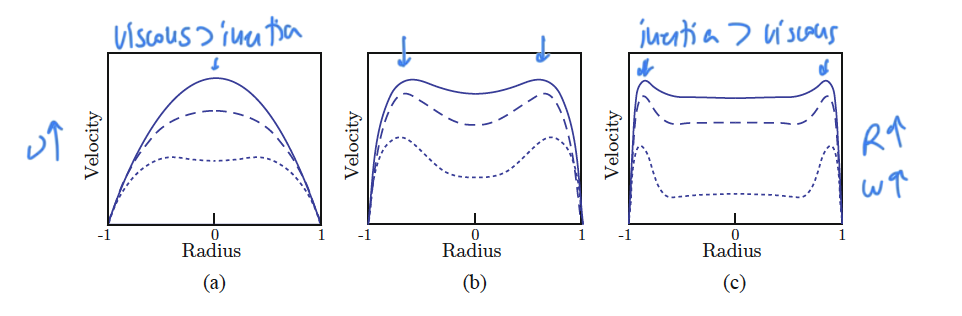
\includegraphics[width=0.85\textwidth]{oscilling-profiles.png}
\caption{Oscillatory velocity profile shape as a function of increasing Womersley number ($\alpha$).
The curves of each plot represent the profile at different phase angles during the oscillation. (a)
$\alpha = 1$. (b) $\alpha = 8$. (c) $\alpha = 15$.}
\end{figure}

\subsection*{Pulsatile Blood Flow}

This corresponds to flow induced by the heart.

Mathematically, it can be described by the superposition of Hagen--Poiseuille flow and oscillatory velocity profiles such as the one 
previously described.

\begin{figure}[H]
\centering
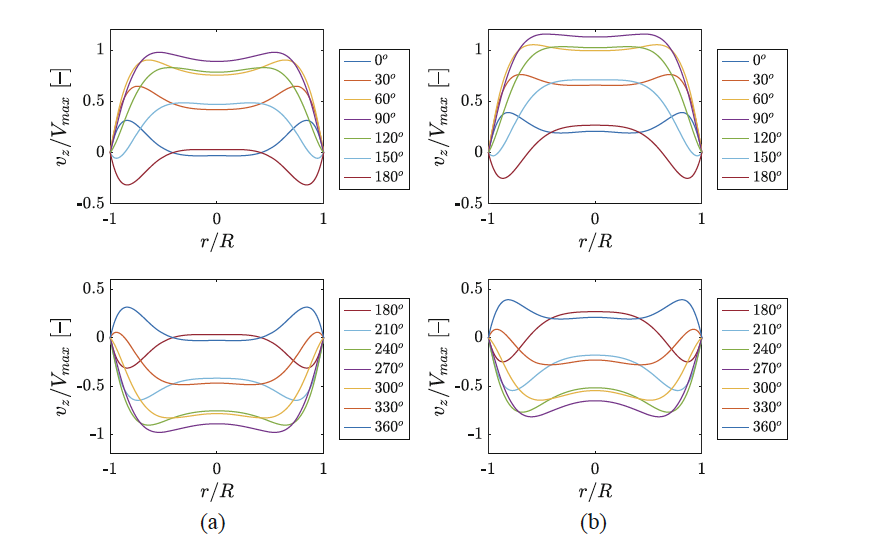
\includegraphics[width=0.85\textwidth]{pulsatile-blood-flow.png}
\caption{Oscillatory (a) and pulsatile (b) velocity profiles for blood flow in the aorta at 70 beats
per minute ($\alpha = 7.5$)}
\end{figure}

As we can see, the oscillating flow is "pushed" towards the direction of the flow. The addition holds the flow from going backwards. 
For higher pulse rate the initial forces dominates over the viscous effects.


\section{Flexible Pipe Flow}

In the cardiovascular system, arteries are not rigid but compliant. This compliance allows the vessels to expand and contract with the pulsatile blood pressure wave, acting as a buffer that maintains continuous flow despite intermittent heartbeats.

Understanding flexible pipe flow is therefore crucial to model:
\begin{itemize}
    \item Pressure wave propagation
    \item Damping and phase lag between pressure and flow
    \item Energy storage and release via wall deformation
\end{itemize}

These properties are particularly important in the aorta and large arteries, where elastic recoil aids in maintaining blood flow during diastole (when the heart is relaxed).


Now we want to get closer to the real world. We leave the rigid pipes behind and take into account the flexible walls, as it actually is for the cardiovascular system.

\medskip

We must now consider the influence of wave speed. In other words, pressure and flow profiles are no longer synchronous.

\medskip

To deal with flexible pipes we need to keep in mind Hooke’s law:

\[
\sigma = \mathcal{E} \, \epsilon
\]
\[
\text{where } \sigma = \text{stress}, \quad \mathcal{E} = \text{elasticity constant}, \quad \epsilon = \text{strain}
\]

\medskip

Arteries are better described as \textit{viscoelastic}, so the stress depends also on the rate of strain:

\[
\sigma_{\text{visco}} = E_1 \, \epsilon + E_2 \, \frac{d\epsilon}{dt}
\]

\medskip

\textbf{Wall balance (subject to strain):}

\[
p_0 x_0 + 2 S_h (r_o - r_i) = \rho_i 2 r_i
\]

\begin{figure}[H]
\centering
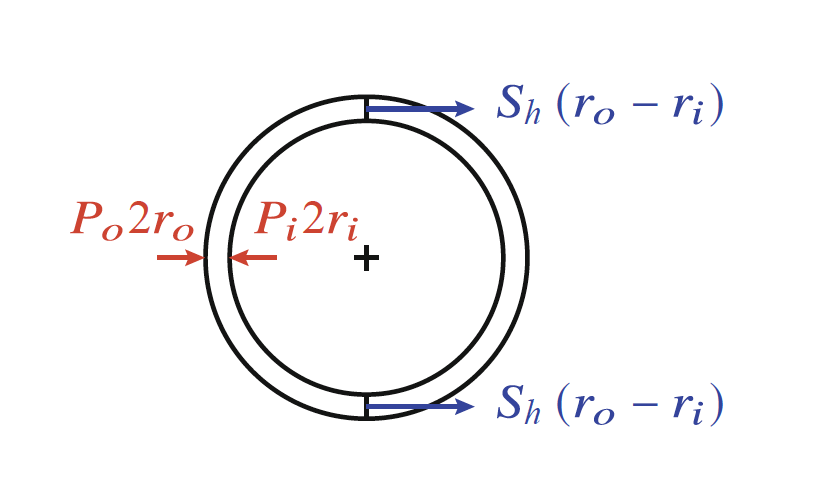
\includegraphics[width=0.6\textwidth]{scheme-flex.png}
\caption{Balance of forces acting on a circular thin-walled vessel due to a transmural pressure (per unit length)}
\end{figure}

\medskip

\textbf{Assuming thin walls:} \( r \sim r_i \sim r_o \)

\[
\delta h_t = p_i - p_0, \qquad S_h \sim \frac{p r}{h_t}
\]

where $h_t=r_0-r_i$.

\textbf{For incremental strains:}

\[
dS_h = d \left( \frac{p r}{h_t} \right)
\]

We can also describe the strain as:

\[
dS_h = \mathcal{E} \frac{dr}{r}
\]

\[
d \left( \frac{p r}{h_t} \right) = \mathcal{E} \frac{dr}{r}
\]

\medskip

\textbf{For incompressible vessels of fixed height (e.g. \( r_0 h_0 \)):}

\[
d \left( \frac{p r^2}{r_0 h_0} \right) = \frac{1}{r_0 h_0} d(p r^2) = \frac{1}{r_0 h_0} \left( 2 r p \, dr + r^2 \, dp \right)
\]

\textbf{Assuming \( dr \approx 0 \) (small strain):}

\[
\mathcal{E} \frac{dr}{r} = \frac{r^2 dp}{r_0 h_0}
\quad \Rightarrow \quad
dp = \mathcal{E} \frac{r_0 h_0}{r^3} dr
\]

\[
\Rightarrow \quad p - p_0 = \frac{\mathcal{E} h_0}{2 r_0} \left( \frac{1}{r_0^2} - \frac{1}{r^2} \right)
\quad \Rightarrow \quad
p - p_0 = \frac{\mathcal{E} h_0}{2 r_0} \left( 1 - \frac{A_0}{A} \right)
\]

\medskip

\textbf{Also:}

\[
\frac{A}{A_0} = \left( 1 - \frac{(p - p_0) 2 r_0}{\mathcal{E} h_0} \right)^{-1}
\]

\medskip

It can be described as a polynomial series with:

\[
c_1 = \frac{2 r_0}{\mathcal{E} h_0}
\]

\[
\frac{A}{A_0} = 1 + c_1 (p - p_0) + \left[ c_1 (p - p_0) \right]^2 + \dots
\]

Neglecting the elements with $c_1$ con orden 2 o superior:

\[
\frac{A}{A_0} = 1 + c_1 (p - p_0) \rightarrow \frac{dA}{dp} = A_0c_1
\]

\[
\frac{dA}{dp} = \pi r_0^2 \frac{2r_0}{E h_0}
\]

\[
\frac{dA}{dp} = \frac{2\pi r_0^2}{E h_0}
\]

Taking as example the human aorta at a distance $L = 200mm$ from the heart.

\begin{figure}[H]
\centering
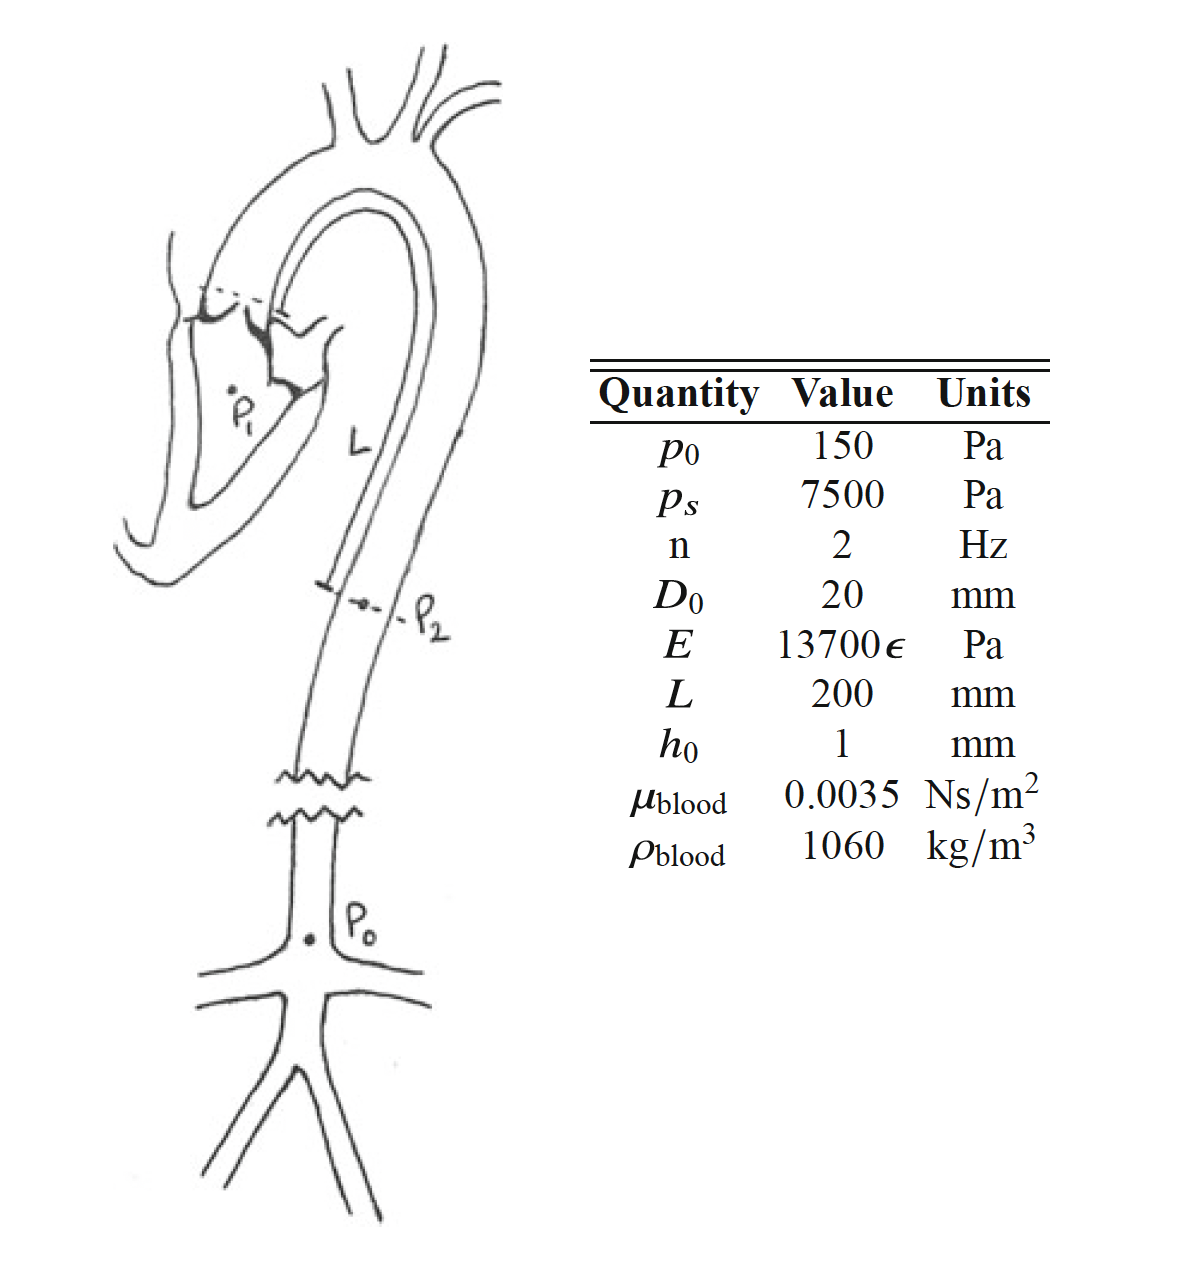
\includegraphics[width=0.6\textwidth]{scheme_cardio.png}
\caption{Schematic diagram and test subject data}
\end{figure}


\subsubsection*{Pressure–Strain Relation and Flow-Driven Deformation}

From the relation:
\[
\frac{dA}{dp} \cdot \frac{\pi D_0}{2} \cdot \frac{dD}{dp} 
\Rightarrow 
\frac{\pi D_0 \, dD}{2 \, dp} = \frac{2 \pi D_0^3}{\mathcal{E} h_0}
\]

\medskip

We can also express the pressure in terms of a strain:

\[
\epsilon = \frac{p - p_0}{p_0}
\]

\medskip

And define a coefficient \( K \) such that:

\[
p = K \, \frac{p(t) - p_0}{p_0}
\]

\medskip

For that case:

\[
K = \frac{p_0}{dp/d\rho} = D_0 \cdot \frac{4 \mathcal{E} h_0}{D_0^2} = \frac{4 \mathcal{E} h_0}{D_0}
\]

\bigskip

\subsubsection*{Rate of Change of Diameter due to Pressure Wave}

The rate of change of the diameter in response to the pressure wave can be determined knowing:

\[
\frac{dD}{dt} = \frac{2}{\pi L} (Q_a - Q_l)
\qquad
Q \equiv \text{flow rate}, \quad Q = \bar{v} S
\]

\medskip

\textbf{Using Hagen–Poiseuille:}

\[
Q_1 = \frac{\pi D^4}{128 \mu L} (p_1 - p_2)
\]

\[
Q_2 = \frac{\pi D^4}{128 \mu L} (p_2 - p_0)
\]

\medskip

\textbf{Finally:}

\[
\frac{dD}{dt} = \frac{1}{64 \mu L^2} D^4 (p_0 + p_1 - 2p_2)
\]

\begin{figure}[H]
\centering
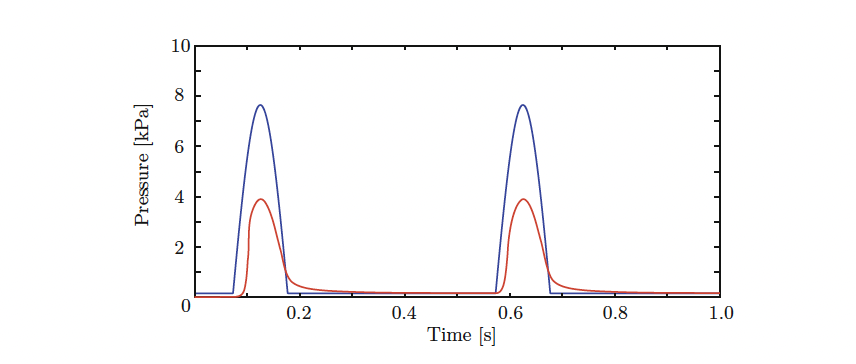
\includegraphics[width=0.85\textwidth]{preassure-fluctuation.png}
\caption{Pressure fluctuations in aorta 200mm downstream from the heart (red curve) as a result
of the signal measured at the heart (blue)}
\end{figure}

\begin{figure}[H]
\centering
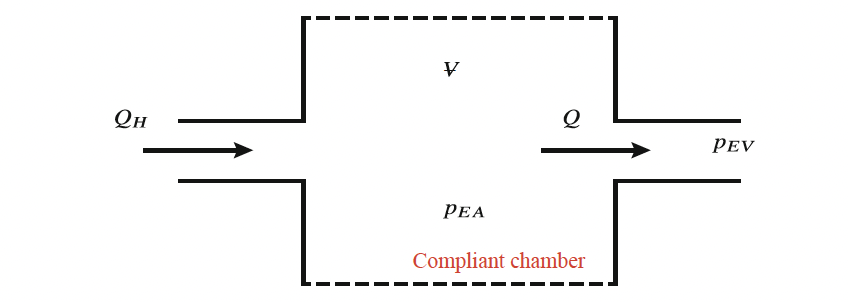
\includegraphics[width=0.85\textwidth]{model-cardiio.png}
\caption{The cardiovascular system is modeled as a simple Windkessel model where the compliant chamber (i.e., its volume $\Vbar$ 
is variable) represents our elastic arteries downstream of the heart.}
\end{figure}


\section*{Conclusion}

In this document, we have progressively built a set of models to describe blood flow in arteries. Beginning with the classical Hagen--Poiseuille 
solution, we incorporated temporal dynamics through an oscillating pressure gradient and culminated in a model accounting for arterial wall 
elasticity.

Each step introduced additional realism and complexity, ultimately leading to a formulation that better reflects physiological conditions such as 
pulsatility, wall compliance, and flow-pressure phase differences. The final model captures essential features of arterial behavior and serves as 
a foundational framework for more advanced cardiovascular simulations.

\end{document}
